%!TEX root =presentation.tex
\subsection[complexity]{Complexity analysis of adjoint method} % (fold)
\label{sec:complexity_analysis_of_adjoint_method}

\begin{frame}[t]\frametitle{Complexity of solving gradient}
    




\begin{block}{Solving adjoint system}
\begin{equation}
    H_x^T \lambda = -J_x
\end{equation}
From previous result, $H_x$ has following properties:

\begin{itemize}
    \item size $|\links|T\times|\links|T$
    \item lower triangular
    \item $card\,H_x = O(|\links|TD_x)$: $D_{x}=\max_{\jn\in\jns}|Inc\left(J\right)\cup Out\left(\jn\right)|$
\end{itemize}

Efficiently solve $\lambda$ via backward-substitution in time $O(card\,H_x)=O(|\links|TD_x)$, or \textbf{linear in $|\links T|$}.
\end{block}

\end{frame}

\begin{frame}[t]\frametitle{Complexity of solving gradient}
    




\begin{block}{Solving $\nabla J$}
\begin{equation}
    \nabla J = \lambda^T H_{\control} + J_{\control}
\end{equation}

From previous result, $H_{\control}$ has following properties:

\begin{itemize}
    \item size $|\links|T\times N_{\control}T$
    \item $card\,H_{\control} = O(|\links|TD_{\control})$: $D_{\control}=\max_{v_{i,k}\in\mathbf{\control}}|\bigcup Inc\left(\jn\right)\cup Out\left(\jn\right):\control_{i,k}\in\mathbf{\control}_{\jn,k}|$
\end{itemize}

Sparse matrix multiplication has total cost $O(D_{\control}N_{\control}T)$, typically of smaller order than solving $H_{\control}$.
\end{block}

\end{frame}


\begin{frame}[t]\frametitle{Complexity of solving gradient}
    
\begin{block}{Total complexity of computing gradient via discrete adjoint}
\begin{equation}
    O(|\mathbf{x}|D_x + |\mathbf{\control}|D_{\control})
\end{equation}
\end{block}

\begin{figure}
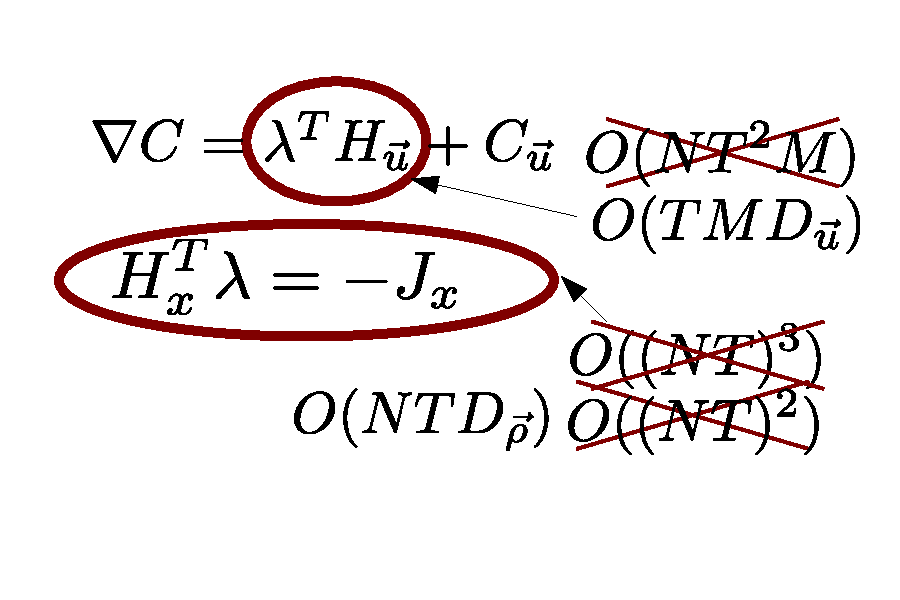
\includegraphics[width=.8\columnwidth]{figs-gen/complexity}
\end{figure}

\end{frame}



% section complexity_analysis_of_adjoint_method (end)